\chapter{$\mathbf{T_{7}^{11}\sqcup T_{2}^{1}}$}
We begin this case by constructing $K_{n}$ for $n \equiv 7 \textrm{ or } 8 \pmod{14}$ and $n\geq 21$ using \textit{joined} copies of $K_{22}$, $K_{21}$, and $K_{14}$. Recall, the \textit{join} of two graphs $G_{1}$ and $G_{2}$ is the graph obtained by adding an edge $\{g_1,g_2\}$ for every vertex $g_1 \in V(G_{1})$ and every vertex of $g_2 \in V(G_{2})$.

Let $t$ be a positive integer and join $t-1$ copies of $K_{14}$ with each other and a lone copy of $K_{21}$. The resulting graph is $K_{14(t-1)+21} \cong K_{14t+7}$. So we can think of $K_{14t+7}$ as $K_{t}$ whose $t$ ``vertices'' consist of $t-1$ copies of $K_{14}$ and $1$ copy of $K_{21}$ and whose edges are the join between them. From now on, we will refer to these ``vertices'' as nodes. Similarly, $K_{14t+8}$ can be constructed as $K_{t}$ whose nodes are $t-1$ copies of $K_{14}$ and $1$ copy of $K_{22}$ and whose edges are the join between them.

We show that $\mathbf{T_{7}^{11}}\sqcup\mathbf{T_{2}^{1}}$ decomposes $K_{n}$ for $n\equiv7 \textrm{ or }8\pmod{14}$ by proving that $K_{22}$, $K_{21}$, $K_{14}$, $K_{22,14}$, $K_{21,14}$, and $K_{14,14}$ are each $\mathbf{T_{7}^{11}}\sqcup\mathbf{T_{2}^{1}}$-decomposable. Notice that these 6 graphs make up the nodes and edges of the $K_{t}$ representations of $K_{14t+7}$ and $K_{14t+8}$ stated in the constructions above.

\noindent The proof of the next theorem was obtained by manipulating a $K_{1,7}$-decomposition of $K_{22}$ by Cain in \cite{bib:Cain}.

\begin{thm}\label{thm:PCstarpath}
    $\mathbf{T_{7}^{11}}\sqcup\mathbf{T_{2}^{1}}$ decomposes $K_{21}$ and $K_{22}$.
\end{thm}

\begin{proof}
     Figures 8 and 9 give $\mathbf{T_{7}^{11}}\sqcup\mathbf{T_{2}^{1}}$-decompositions of $K_{21}$ and $K_{22}$, respectively.%The table will contain ad-hoc decompositions of $K_{21}$ and $K_{22}$. The construction for $K_{21}$ results from plucking edges off of Pauline Cain's $7$-star decomposition of $K_{21}$ and mixing them around, and The construction for $K_{22}$ results from adding three stars centered at $\infty$ and three lone paths beginning at $\infty$. Once again, edges are plucked off and mixed around to make this work.
\end{proof}
\newpage
\begin{thm} \label{thm:K_n,7}
    $\mathbf{T_{7}^{11}}\sqcup\mathbf{T_{2}^{1}}$ decomposes $K_{n,7}$ for all $n\geq 2$.
\end{thm}

\begin{proof}
    Consider $K_{n,7}$ where $n\geq 2$. Take the partite set of $n$ vertices to be $\ZZ_{n}$ and color them white. Similarly, take the partite set of $7$ vertices to be $K_{7}$ and color them black. Naturally we refer to \textit{white-black} vertices $uv$ in $K_{n,7}$ via $(u,v)\in \ZZ_{n}\times\ZZ_{7}$ and vice versa. Finally, let $E_{i}=\{(i,0)\}\sqcup (\{i+1\}\times \{1,\hdots,6\})$ and $G_{i}\subset K_{n,7}$ be the subgraph induced by $E_{i}$ for each $i\in \ZZ_{n}$. Note that $G_{i}\cong \mathbf{T_{7}^{11}}\sqcup\mathbf{T_{2}^{1}}$ for all $i\in \ZZ_{n}$.

    \begin{figure}[H]
        \centering
        \documentclass{standalone}
\usepackage{amsmath,mathabx}
\usepackage{tikz}
\usetikzlibrary{positioning}
\begin{document}
    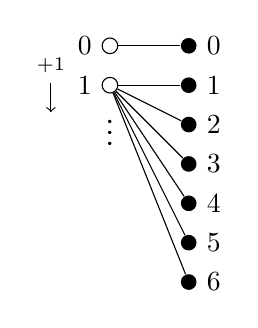
\begin{tikzpicture}[scale=0.5]
        %white
        \node[fill=white,draw =black, circle, inner sep=2pt, label=left:{\textcolor{black}{$0$}}] (w0) at (0,0) {};
        \node[fill=white,draw = black, circle, inner sep=2pt, label=left:{\textcolor{black}{$1$}}] (w1) at (0,-1) {};
        \node at (0,-2) {\large $\vdots$};

        %\node[draw=black, fill=white, circle, inner sep=1pt] (circ) at (-1.5,-0.5) {};
        \node (p1) at (-1.5,-0.5) {\scriptsize +1};
        \draw[->] ([yshift=0pt] p1.south) -- ++(0, -0.75);
        %black nodes
        \node[fill=black, circle, inner sep=2pt, label=right:{\textcolor{black}{$0$}}] (b0) at (2,0) {};
        \node[fill=black, circle, inner sep=2pt, label=right:{\textcolor{black}{$1$}}] (b1) at (2,-1) {};
        \node[fill=black, circle, inner sep=2pt, label=right:{\textcolor{black}{$2$}}] (b2) at (2,-2) {};
        \node[fill=black, circle, inner sep=2pt, label=right:{\textcolor{black}{$3$}}] (b3) at (2,-3) {};
        \node[fill=black, circle, inner sep=2pt, label=right:{\textcolor{black}{$4$}}] (b4) at (2,-4) {};
        \node[fill=black, circle, inner sep=2pt, label=right:{\textcolor{black}{$5$}}] (b5) at (2,-5) {};
        \node[fill=black, circle, inner sep=2pt, label=right:{\textcolor{black}{$6$}}] (b6) at (2,-6) {};
        \node at (0,-2) {\large $\vdots$};

        \draw[draw=black, shorten >=0pt, shorten <=0pt] (w0) -- (b0);
        \draw[draw=black, shorten >=0pt, shorten <=0pt] (w1) -- (b1);
        \draw[draw=black, shorten >=0pt, shorten <=0pt] (w1) -- (b2);
        \draw[draw=black, shorten >=0pt, shorten <=0pt] (w1) -- (b3);
        \draw[draw=black, shorten >=0pt, shorten <=0pt] (w1) -- (b4);
        \draw[draw=black, shorten >=0pt, shorten <=0pt] (w1) -- (b5);
        \draw[draw=black, shorten >=0pt, shorten <=0pt] (w1) -- (b6);
    \end{tikzpicture}
\end{document}
        \caption{$G_{0}$ in a generating presentation of the $\mathbf{T_{7}^{11}}\sqcup\mathbf{T_{2}^{1}}-$decomposition of $K_{n,7}$.}
        \label{fig:enter-label}
    \end{figure}

    \noindent Notice that $E_{i}\cap E_{j}=\emptyset$ if $i\neq j$, so by definition all distinct $G_{i}$'s are pairwise edge disjoint. Lastly,
    
    $$\bigcup_{i\in \ZZ_{n}} E_{i}=[\bigcup_{i\in \ZZ_{n}} \{(i,0)\}]\sqcup [\bigcup_{i\in \ZZ_{n}} (\{i+1\}\times \{1,\hdots, 6\})]=[\ZZ_{n}\times \{0\}]\sqcup [\ZZ_{n}\times \{1,\hdots, 6\}]=\ZZ_{n}\times \ZZ_{7}$$.
    
    \noindent So $G_{0}\sqcup \cdots \sqcup G_{n-1}=K_{n,7}$ and $\{G_{i}\mid i\in \ZZ_{n}\}$ is a $\mathbf{T_{7}^{11}}\sqcup\mathbf{T_{2}^{1}}-$decomposition of $K_{n,7}$. Furthermore, it is generated by developing the white nodes of $G_{0}$ by $1$.
\end{proof}

%old proof:

    %Take the partite set of $n$ nodes to be $\ZZ_{n}$ and color them white. Then, take the other partite set of $7$ nodes to be $\ZZ_{7}$ and color them black. Notice that $|E(K_{n,7})|=|\ZZ_{n}\oplus \ZZ_{7}|=7n$. So let us refer to edges of $K_{n,7}$ as elements of $\ZZ_{n}\oplus \ZZ_{7}$ and vice versa. Note that since $n\geq 2, (1,0)\neq (0,0)$.

    %Now, let $E_{i}= (i,0)+\{(0,0),(1,1),(1,2),\hdots,(1,6)\}$ for each $i\in \ZZ_{n}$ and $F_{i}$ be the subgraph induced by $E_{i}$. Since each $F_{i}$ contains a path $(i,0)$ which is vertex disjoint from the star centered at the white $i+1$, it must be isomorphic to $\mathbf{T_{7}^{11}}\sqcup\mathbf{T_{2}^{1}}$.

    %note to self: originally I thought of E_i's as (i,0) + (\{(0,0)\}\cup [(1,0)+[\langle (0,1)\rangle\setminus \{(0,0)\}]])

    %the union expression at the end is messy. However, the point of using groups here is basically that when we use generator notation we can swallow things up to get simpler things in terms of generators and it works out nicely here.
    
    %\noindent Suppose that there exist distinct $i,j\in \ZZ_{n}$ such that $E_{i}\cap E_{j}\neq \emptyset$. But then we have that $(i,0)=(j,0)$ or $(i+1,a)=(j+1,b)$ for some $a,b\in \ZZ_{7}$, which is impossible. So all distinct $E_{i}$'s are pairwise disjoint, and therefore all distinct $F_{i}$'s are pairwise edge-disjoint. Lastly, $\bigcup_{i\in \ZZ_{n}} E_{i}=\langle (1,0)\rangle + [\{(0,0)\}\cup [(1,0)+\langle (0,1)\rangle] \setminus \{(1,0)\}]=\langle (1,0)\rangle + \langle (0,1)\rangle = \langle (1,0),(0,1)\rangle = \ZZ_{n}\oplus \ZZ_{7}$. Therefore, $\bigcup_{i\in \ZZ_{n}} F_{i} = K_{n,7}$. \\

\begin{corollary}\label{cor:starpathbi}
    $\mathbf{T_{7}^{11}}\sqcup\mathbf{T_{2}^{1}}$ decomposes $K_{22,14}$, $K_{21,14},\text{ and }K_{14,14}$.
\end{corollary}

\begin{proof}
    $\mathbf{T_{7}^{11}}\sqcup\mathbf{T_{2}^{1}}$ decomposes $K_{7,7}$ and $K_{8,7}$ by Theorem \ref{thm:K_n,7}. $K_{14,14}$ can be expressed as the edge-disjoint union of four copies of $K_{7,7}$, $K_{21,14}$ can be expressed as the edge-disjoint union of six copies of $K_{7,7}$, and $K_{22,14}$ can be expressed as the edge-disjoint union of two copies of $K_{8,7}$ and four copies of $K_{7,7}$. Therefore, $\mathbf{T_{7}^{11}}\sqcup\mathbf{T_{2}^{1}}$ decomposes them all.
\end{proof}

\begin{thm}
$\mathbf{T_{7}^{11}}\sqcup\mathbf{T_{2}^{1}}$ decomposes $K_{14t+7}$ and $K_{14t+8}$ where $t$ is a positive integer. 
\end{thm}
\begin{proof}
$\mathbf{T_{7}^{11}}\sqcup\mathbf{T_{2}^{1}}$ decomposes $K_{14}$ by Theorem \ref{thm:sigma plus minus}, $K_{22,14}$, $K_{21,14},\text{ and }K_{14,14}$ by Corollary \ref{cor:starpathbi}, and lastly $K_{22},K_{21}$ by Theorem \ref{thm:PCstarpath}.
\newline\newline
Therefore, $\mathbf{T_{7}^{11}}\sqcup\mathbf{T_{2}^{1}}$ decomposes the join of $(t-1)$ copies of $K_{14}$ with each other and $1$ copy of $K_{21}$, which is isomorphic to $K_{14t+7}$. Similarly $\mathbf{T_{7}^{11}}\sqcup\mathbf{T_{2}^{1}}$ decomposes the join of $(t-1)$ copies of $K_{14}$ with each other and $1$ copy of $K_{22}$ which is isomorphic to $K_{14t+8}$.
\end{proof}